\section{Расчёт трудоёмкости проекта} \label{economics_laboriousness}
% \addcontentsline{toc}{chapter}{Понятие системы электронного документооборота}  % Добавляем его в оглавление

Общие затраты труда на разработку и ПО определим следующим образом:
\begin{equation}
  \label{eq:common_laboriousness}
Q_p = \sum_{i} T_i,
\end{equation}
где $T_i$ --- затраты труда на выполнение $i$\ndashго этапа проекта.

Используя метод экспертных оценок, вычислим ожидаемую продолжительность работ $T$ каждого этапа по формуле:
\begin{equation}
  \label{eq:work_duration}
T = \frac {3 \cdot T_{MIN} + 2 \cdot T_{MAX}} {5},
\end{equation}
где $T_{MAX}$ и $T_{MIN}$ – максимальная и минимальная продолжительность работы. Они назначаются в соответствии с экспертными оценками, а ожидаемая продолжительность работы рассчитывается как математическое ожидание для $\beta$\ndash распределения.

\vspace{\baselineskip}
Полный перечень работ с разделением их по этапам приведён в таблице \ref{table:works}.
\begin{center}
 \renewcommand\multirowsetup{\centering}
 \begin{longtable}[h]{| c | >{\centering}m{3cm} | c | >{\centering}m{5cm} | >{\centering}m{1cm} | >{\centering}m{1cm} | >{\centering}m{1cm} | >{\centering}m{1cm} |}
  \captionsetup{justification=raggedright}
  \caption{Распределение работ по этапам} \label{table:works} \tabularnewline
  \hline

\rowcolor{Gray} №  & Этап & № работы &  Содержание работы & $T_{MIN}$, чел / часы & $T_{MAX}$, чел / часы & $T$, чел / часы & $T$, чел / дни \tabularnewline \hline \endfirsthead   \hline
 \multicolumn{8}{|c|}{\small\slshape (продолжение таблицы \ref{table:works})}        \tabularnewline \hline
 \rowcolor{Gray} №  & Этап & № работы &  Содержание работы & $T_{MIN}$, чел / часы & $T_{MAX}$, чел / часы & $T$, чел / часы & $T$, чел / дни \tabularnewline \hline
                                              \endhead        \hline
 % \multicolumn{8}{|r|}{\small\slshape продолжение следует}  \tabularnewline \hline
                                              \endfoot        \hline
                                              \endlastfoot

\multirow{5}{*}{1} 	& \multirow{5}{3cm}{Разработка технических требований}	& 1 & Получение задания, анализ полученных требований к разрабатываемому ПО		& 8 & 8	& 8	& 1 \tabularnewline \cline{3-8}
 	& & 2 & Разработка и утверждение ТЗ 	& 24 & 24 & 24 & 3 \tabularnewline \cline{3-8}
 	& & 3 & Анализ предметной области и существующих решений & 24 & 44 & 32  & 4 \tabularnewline \cline{3-8}
 	& & 4 & Анализ потоков данных в процессе электронного документооборота & 72 & 92 & 80 & 10 \tabularnewline \hline

\multirow{2}{*}{2} & \multirow{2}{3cm}{Разработка алгоритмов} & 5 & Разработка общей структуры ПО и пользовательского интерфейса & 24 & 44 & 32 & 4 \tabularnewline \cline{3-8}
	& & 6 & Разработка алгоритмов, структуры входных и выходных данных & 64 & 84 & 72 & 9 \tabularnewline \hline

\multirow{2}{*}{3} & \multirow{2}{3cm}{Разработка программных модулей} & 7 & Реализация пользовательского интерфейса & 32 & 52 & 40 & 5 \tabularnewline \cline{3-8}
	& & 8 & Программная реализация модулей защищенной обработки, передачи и хранения информации & 72 & 92 & 80 & 10 \tabularnewline \hline \pagebreak

\multirow{6}{*}{4} & \multirow{6}{2.5cm}{Тестирование и отладка разрабатываемого ПО} & & & & & & \tabularnewline
  & & 9 & Тестирование ПО & 64 & 84 & 72 & 9 \tabularnewline
  & & & & & & & \tabularnewline \cline{3-8}
	& & & & & & & \tabularnewline
	& & 10 & Внесение изменений в ПО & 32 & 52 & 40 & 5 \tabularnewline
	& & & & & & & \tabularnewline \hline

5 & Разработка документации & 11 & Разработка программной и эксплуатационной документации & 64 & 84 & 72 & 9 \tabularnewline \hline

\multicolumn{4}{|l|}{Итого $Q_P$:} & \multicolumn{3}{|l|}{616} & 77 \tabularnewline \hline

\end{longtable}
\end{center}

\begin{equation}
  \label{eq:common_laboriousness_result}
Q_P = Q_{\textrm{ОЖ}} = 77 (\textrm{чел/дней}) = 616 (\textrm{чел/час}).
\end{equation}
\FloatBarrier

\section{Определение численности исполнителей} \label{workers}

Для оценки возможности выполнения проекта имеющимся в распоряжении разработчика штатным составом исполнителей нужно рассчитать их среднее количество, которое при реализации проекта разработки и внедрения ПО определяется соотношением:
\begin{equation}
  \label{eq:common_workers}
N = \frac {Q_P} {F},
\end{equation}
где $Q_P$ -- затраты труда на выполнение проекта (разработка и внедрение ПО), а $F$ -- фонд рабочего времени, который определяется по формуле:
\begin{equation}
  \label{eq:time_fund_month_common}
F_M = T \cdot \frac {t_P \cdot (D_K - D_B - D_\textrm{П})} {12},
\end{equation}
где $T$ -- время выполнения проекта в месяцах, $t_P$ -- продолжительность рабочего дня, $D_K$ -- общее число дней в году, $D_B$ -- число выходных дней в году, $D_\textrm{П}$ -- число праздничных дней в году.

\vspace{\baselineskip}
Таким образом, фонд времени в текущем месяце 2014 года составляет
\begin{equation}
  \label{eq:time_fund_month}
F_M = \frac {8 \cdot (365 - 104 - 14)} {12} = 165 \textrm{ часов/мес}.
\end{equation}

Время выполнения проекта $T = 3,5$ (месяца).

\vspace{\baselineskip}
Величина фонда рабочего времени составляет:
\begin{equation}
  \label{eq:time_fund}
F = T \cdot F_M = 577,5 \textrm{ ч}.
\end{equation}

Затраты труда на выполнения проекта были рассчитаны в предыдущем разделе, их величина равна $616 \textrm{ чел/час}$. В соответствии с этими данными и выражением (\ref{eq:common_workers}), среднее количество исполнителей равно:
\begin{equation}
  \label{eq:workers_avg}
N = \frac {616} {577,5} = 1,07.
\end{equation}

Округляя до большего, получим число исполнителей проекта $N = 2$.            % Определение численности исполнителей
\subsection{Построение сетевого графика} \label{net_graph}

Для определения временных затрат и трудоемкости разработки ПО используем метод сетевого планирования. Метод сетевого планирования позволяет установить единой схемой связь между всеми работами в виде наглядного и удобного для восприятия изображения (сетевого графика), представляющего собой информационно-динамическую модель, позволяющую определить продолжительность и трудоёмкость, как отдельных этапов, так и всего комплекса работ в целом.

\vspace{\baselineskip}
Составление сетевой модели включает в себя оценку степени детализации комплекса работ и определения логической связи между отдельными работами.
С этой целью составляется перечень всех основных событий и работ. В перечне указываются кодовые номера событий, наименования событий в последовательности от исходного к завершающему, кодовые номера работ, перечень всех работ, причём подряд указываются все работы, которые начинаются после наступления данного события.

\vspace{\baselineskip}
Основные события и работы проекта представлены в таблице \ref{table:events}.


\begin{center}
\renewcommand\multirowsetup{\centering}
\begin{longtable}[h]{| >{\centering}m{1cm} | >{\centering}m{4cm} | >{\centering}m{1.5cm} | >{\centering}m{5cm} | >{\centering}m{1cm} | >{\centering}m{1cm} |}
  \captionsetup{justification=raggedright}
	\caption{Основные события и работы проекта} \label{table:events} \tabularnewline
  \hline


\rowcolor{Gray}   $N_i$  &   Наименование события &  Код работы &   Работа &   $t$, чел / час &   $t$,  чел / день \tabularnewline \hline \endfirsthead   \hline
 \multicolumn{6}{|c|}{\small\slshape (продолжение таблицы \ref{table:events})}        \tabularnewline \hline
 \rowcolor{Gray}   $N_i$  &   Наименование события &   Код работы &    Работа &  $t$, чел / час &  $t$,  чел / день               \tabularnewline \hline
                                              \endhead        \hline
 % \multicolumn{6}{|r|}{\small\slshape продолжение следует}  \tabularnewline \hline
                                              \endfoot        \hline
                                              \endlastfoot


 % \rowcolor{Gray}  $N_i$  &  Наименование события &  Код работы &   Работы &  $t$, чел / час &  $t$,  чел / день \tabularnewline \hline

 0 & Разработка ПО начата & 0-1 & Получение задания, анализ полученных требований к разрабатываемому ПО & 8 & 1 \tabularnewline \hline

 1 & Анализ полученных требований к разрабатываемому ПО проведен & 1-2 & Разработка и утверждение ТЗ & 24 & 3 \tabularnewline \hline
 
 2 & ТЗ разработано и утверждено & 2-3 & Анализ предметной области и существующих решений & 32 & 4 \tabularnewline \hline
 
 3 & Анализ предметной области и существующих решений проведён & 3-4 & Анализ потоков данных в процессе электронного документооборота & 80 & 10 \tabularnewline \hline
 
 4 & Анализ потоков данных в процессе электронного документооборота проведён & 4-5 & Разработка общей структуры ПО и пользовательского интерфейса & 32 & 4 \tabularnewline \hline
 
 5 & Разработка общей структуры ПО и пользовательского интерфейса завершена & 5-6 & Разработка алгоритмов, структуры входных и выходных данных & 72 & 9 \tabularnewline \hline %\pagebreak
 
\multirow{2}{1cm}{6} & \multirow{2}{4cm}{Разработка алгоритмов, структуры входных и выходных данных завершена} & 6-7 & Реализация пользовательского интерфейса & 40 & 5 \tabularnewline \cline{3-6}
& & 6-8 & Программная реализация модулей защищенной обработки, передачи и хранения информации & 80 & 10 \tabularnewline \hline

7 & Реализация пользовательского интерфейса завершена & 7-8 & Фиктивная работа & 0 & 0 \tabularnewline \hline

\multirow{6}{1cm}{8} & \multirow{6}{4cm}{Программная реализация модулей защищенной обработки, передачи и хранения информации завершена} & & & & \tabularnewline
 & & & & & \tabularnewline
 & & 8-9 & Тестирование ПО & 64 & 8 \tabularnewline 
 & & & & & \tabularnewline
 & & & & & \tabularnewline \cline{3-6} 
 & & & & & \tabularnewline
 & & 8-10 & Разработка документации & 80 & 10 \tabularnewline
 & & & & & \tabularnewline \hline

 9 & Тестирование ПО завершено & 9-11 & Внесение изменений в ПО & 40 & 5 \tabularnewline \hline

 10 & Документация разработана & 1-12 & Фиктивная работа & 0 & 0 \tabularnewline \hline

 11 & Внесение изменений в ПО закончено & 11-12 & Фиктивная работа & 0 & 0 \tabularnewline \hline

 12 & Разработка ПО закончена & --- & --- & --- & --- \tabularnewline \hline
\end{longtable}
\end{center}


Рассчитанные оставшиеся параметры элементов сети (сроки наступления событий, резервы времени событий, полный и свободный резервы времени работ) приведены в таблице \ref{table:time_per_work}.
\begin{table} [h!]
  
  \captionsetup{justification=raggedright}
  \caption{Временные затраты на каждый этап работы}\label{table:time_per_work}
 \begin{center}
  \begin{tabular}{| c | >{\centering}m{1.5cm} | >{\centering}m{1.5cm} | >{\centering}m{1.5cm} | >{\centering}m{1.5cm} | >{\centering}m{1.5cm} | >{\centering}m{1.5cm} | >{\centering}m{1.5cm} |}
  \hline
 \rowcolor{Gray} $N_i$  & Код работы $i-j$ & $t_{i-j}$, чел / день &  $T_i^P$, чел / день & $T_i^\textrm{П}$, чел / день & $R_i$, чел / день & $R_{i-j}^\textrm{П}$, чел / день & $R_{i-j}^C$, чел / день \tabularnewline \hline

 0 & 0-1 & 1 & 0 & 0 & 0 & 0 & 0 \tabularnewline \hline
 1 & 1-2 & 3 & 1 & 1 & 0 & 0 & 0 \tabularnewline \hline
 2 & 2-3 & 4 & 4 & 4 & 0 & 0 & 0 \tabularnewline \hline
 3 & 3-4 & 10 & 8 & 8 & 0 & 0 & 0 \tabularnewline \hline
 4 & 4-5 & 4 & 18 & 18 & 0 & 0 & 0 \tabularnewline \hline
 5 & 5-6 & 9 & 22 & 22 & 0 & 0 & 0 \tabularnewline \hline
 \multirow{2}{*}{6} & 6-7 & 5 & \multirow{2}{*}{31} & \multirow{2}{*}{31} & \multirow{2}{*}{0} & 5 & 0 \tabularnewline \cline{2-3} \cline{7-8}
  & 6-8 & 10 & & & & 0 & 0 \tabularnewline \hline
  7 & 7-8 & 0 & 36 & 41 & 5 & 0 & 0 \tabularnewline \hline
\multirow{2}{*}{8} & 8-9 & 8 & \multirow{2}{*}{41} & \multirow{2}{*}{41} & \multirow{2}{*}{0} & 0 & 0 \tabularnewline \cline{2-3} \cline{7-8}
  & 8-10 & 10 & & & & 3 & 0 \tabularnewline \hline
  9 & 9-11 & 5 & 49 & 49 & 0 & 0 & 0 \tabularnewline \hline
  10 & 10-12& 0 & 51 & 54 & 3 & 0 & 0 \tabularnewline \hline
  11 & 11-12 & 0 & 54 & 54 & 0 & 0 & 0 \tabularnewline \hline
  12 & - & - & 54 & 54 & 0 & 0 & 0 \tabularnewline \hline
   \end{tabular}
 \end{center}
\end{table}

Здесь \textbf{ранний срок совершения события} $T_j^P$ определяет минимальное время, необходимое для выполнения всех работ, предшествующих данному событию и равен продолжительности наибольшего из путей, ведущих от исходного события к рассматриваемому:
\begin{equation}
  \label{eq:T_j^P}
T_j^P = max \{ T_i^P + t_{i-j}\}.
\end{equation}

\textbf{Поздний срок совершения события} $T_i^\textrm{П}$ – это максимально допустимое время наступления данного события, при котором сохраняется возможность соблюдения ранних сроков наступления последующих событий. Поздние сроки равны разности между поздним сроком совершения $j$-го события и продолжительностью работы $i-j$:
\begin{equation}
  \label{eq:T_j_late}
T_i^\textrm{П} = min \{ T_j^\textrm{П} - t_{i-j}\}.
\end{equation}

\textbf{Критический путь} – это максимальный путь от исходного события до завершения проекта. Его определение позволяет обратить внимание на перечень событий, совокупность которых имеет нулевой резерв времени.

Все события в сети, не принадлежащие критическому пути, имеют \textbf{резерв времени} $R_i$,  показывающий, на какой предельный срок можно задержать наступление этого события, не увеличивая сроки окончания работ:
\begin{equation}
  \label{eq:R_i}
R_i = T_i^\textrm{П} - T_i^P.
\end{equation}

\textbf{Полный резерв времени работы} $R_{i-j}^\textrm{П}$ и \textbf{свободный резерв времени} $R_{i-j}^C$ работы можно определить, используя следующие соотношения:
\begin{equation}
  \label{eq:R_ij_full}
R_{i-j}^\textrm{П} = T_j^\textrm{П} - T_i^P - t_{i-j}.
\end{equation}
\begin{equation}
  \label{eq:R_ij^C}
R_{i-j}^C = T_j^P - T_i^P - t_{i-j}.
\end{equation}

Полный резерв работы показывает максимальное время, на которое можно увеличить длительность работы или отсрочить ее начало, чтобы не нарушился срок завершения проекта в целом. Свободный резерв работы показывает максимальное время, на которое можно увеличить продолжительность работы или отсрочить ее начало, не меняя ранних сроков начала последующих работ.

Сетевой график приведён на рис. \ref{img:net_graph}.

\begin{figure} [h] 
  \center
  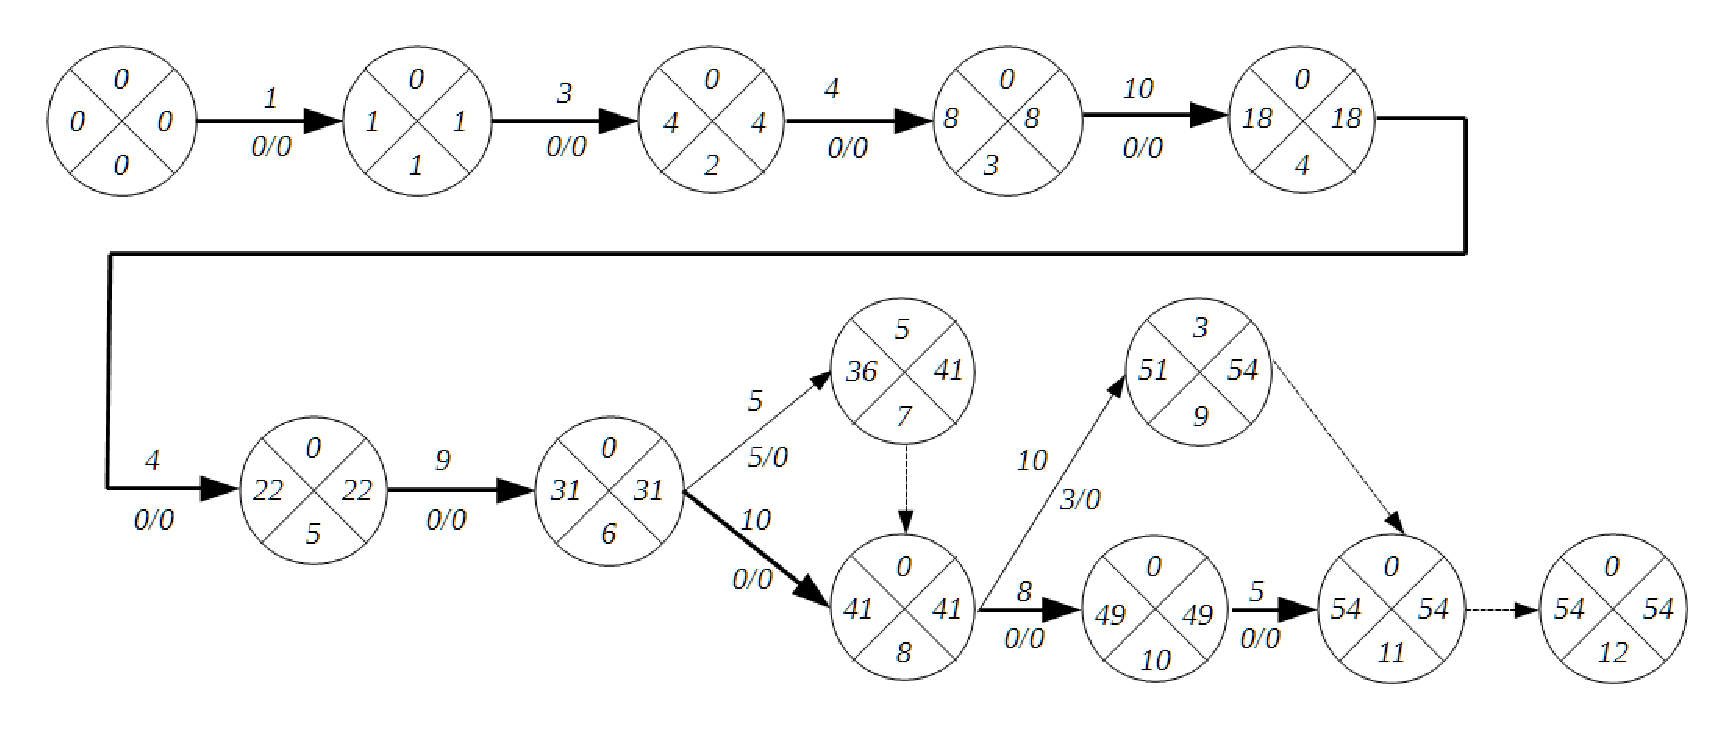
\includegraphics [scale=0.6] {netgraph}
  \caption{Сетевой график выполнения работ} 
  \label{img:net_graph}  
\end{figure}         % Построение сетевого графика
\subsection{Диаграмма Ганта} \label{gant}

Для иллюстрации последовательности проводимых работ приведем диаграмму Ганта данного проекта, на которой по оси $X$ изображены календарные дни от начала до конца проекта, а по оси $Y$ – выполняемые этапы работ.
Диаграмма Ганта приведена на рисунке \ref{img:gant_diagram}. Занятость исполнителей приведена в таблице \ref{table:workers_dates}.

\begin{figure} [h] 
  \center
  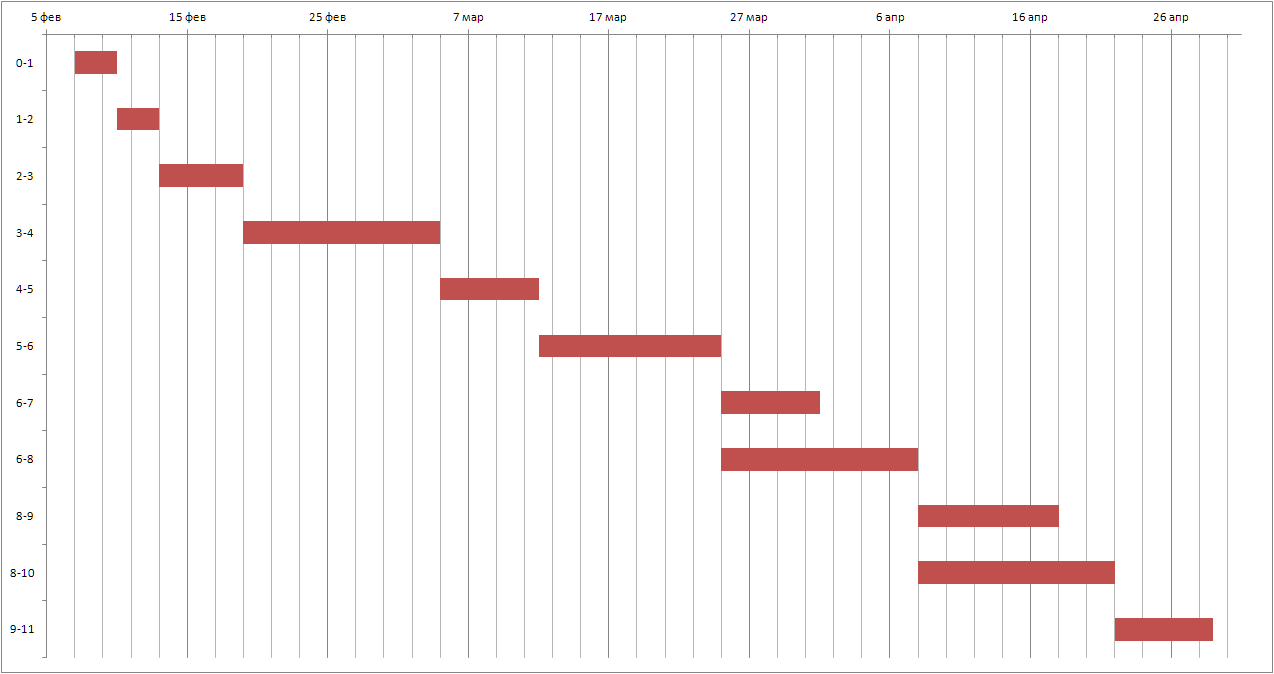
\includegraphics [scale=0.5] {gantt}
  \caption{Диаграмма Ганта проводимых работ} 
  \label{img:gant_diagram}  
\end{figure}

\begin{center}
 \renewcommand\multirowsetup{\centering}
 \begin{longtable}[h]{| >{\centering}m{2cm} | >{\centering}m{4cm} | >{\centering}m{4cm} | >{\centering}m{5cm}|}
	\captionsetup{justification=raggedright}
	\caption{Занятость исполнителей} \label{table:workers_dates} \tabularnewline
	\hline

 \rowcolor{Gray}  Код работы  & Дата начала & Дата окончания &  Исполнитель \tabularnewline \hline \endfirsthead   \hline
 \multicolumn{4}{|c|}{\small\slshape (продолжение таблицы \ref{table:workers_dates})}        \tabularnewline \hline
 \rowcolor{Gray}  Код работы  & Дата начала & Дата окончания &  Исполнитель \tabularnewline \hline
                                              \endhead        \hline
 % \multicolumn{3}{|r|}{\small\slshape продолжение следует}  \tabularnewline \hline
                                              \endfoot        \hline
                                              \endlastfoot

0-1 & 07.02.2014 & 07.02.2014 & Ведущий программист \tabularnewline \hline
1-2 & 09.02.2014 & 12.02.2014 & Ведущий программист \tabularnewline \hline
2-3 & 13.02.2014 & 18.02.2014 & Ведущий программист \tabularnewline \hline
3-4 & 19.02.2014 & 04.03.2014 & Ведущий программист \tabularnewline \hline
4-5 & 05.03.2014 & 11.03.2014 & Ведущий программист \tabularnewline \hline
5-6 & 12.03.2014 & 24.03.2014 & Ведущий программист \tabularnewline \hline
6-7 & 25.03.2014 & 31.03.2014 & Программист \tabularnewline \hline
6-8 & 25.03.2014 & 07.04.2014 & Ведущий программист \tabularnewline \hline
8-9 & 08.04.2014 & 17.04.2014 & Программист \tabularnewline \hline
8-10 &08.04.2014 & 21.04.2014 & Ведущий программист \tabularnewline \hline
9-11 & 22.04.2014 & 28.04.2014 & Ведущий программист \tabularnewline \hline
\end{longtable}
\end{center}

\FloatBarrier             % Диаграмма Ганта
\subsection{Анализ структуры затрат проекта} \label{costs_analysus}

Затраты на выполнение проекта могут быть представлены в виде сметы затрат, включающей в себя следующие статьи:
\begin{itemize}
	\item заработная плата исполнителям;
	\item отчисления на социальные нужды;
	\item материальные затраты;
	\item амортизационные затраты;
	\item прочие затраты.
\end{itemize}    % Анализ структуры затрат проекта
\subsection{Затраты на выплату заработной платы} \label{salary}

Затраты на выплату исполнителям заработной платы линейно связаны с трудоемкостью и определяется следующим соотношением:
\begin{equation}
  \label{eq:salary}
C_\textrm{ЗАРП} = C_\textrm{З.ОСН} + C_\textrm{З.ДОП} + C_\textrm{З.ОТЧ},
\end{equation}
где $C_\textrm{З.ОСН}$ --- основная заработная плата, $C_\textrm{З.ДОП}$ --- дополнительная заработная плата, $C_\textrm{З.ОТЧ}$ --- отчисление с заработной платы.

\vspace{\baselineskip}
Расчёт основной заработной платы (оплаты труда непосредственных исполнителей):
\begin{equation}
  \label{eq:salary_counting}
C_\textrm{З.ОСН} = T_\textrm{ЗАН} \times O_\textrm{ДН},
\end{equation}
где $T_\textrm{ЗАН}$ --- число дней, отработанных исполнителем проекта, а $O_\textrm{ДН}$ --- днейвной оклад исполнителя, который при 8-часовом рабочем дней рассчитывается по формуле:
\begin{equation}
  \label{eq:worker_fee}
O_\textrm{ДН} = \frac {O_\textrm{МЕС} \cdot 8} {F_M},
\end{equation}
где $O_\textrm{МЕС}$ --- месячный оклад, а $F_M$ --- месячный фонд рабочего времени (\ref{eq:time_fund_month_common}).

\vspace{\baselineskip}
С учетом налога на доходы физических лиц размер оклада увеличивается:
\begin{equation}
  \label{eq:worker_fee_with_taxes}
O_\textrm{МЕС} = O \cdot (1 + \frac {H_\textrm{ДФЛ}} {100}),
\end{equation}
где $O$ --- <<чистый>> оклад, $H_\textrm{ДФЛ}$ --- налог на доходы физических лиц ($13\%$).

\vspace{\baselineskip}
Сведем результаты расчета в таблицу с перечнем исполнителей и их месячных и дневных окладов, а также времени участия в проекте и рассчитанной основной заработной платой каждого исполнителя (таблица \ref{table:fee_all_workers}).

\begin{table} [h!]
  \captionsetup{justification=raggedright}
  \caption{Заработная плата исполнителей}\label{table:fee_all_workers}
 \begin{center}
  \begin{tabular}{| c | >{\centering}m{3cm} | >{\centering}m{2.5cm} | >{\centering}m{2.5cm} | >{\centering}m{2.5cm} | >{\centering}m{2.5cm} |}
  \hline
 \rowcolor{Gray} №  & Должность & <<Чистый>> оклад, руб. & Дневной оклад, руб. &  Трудозатраты, чел-дни & Затраты на зарплату, руб. \tabularnewline \hline

 1 & Ведущий программист & 60 000 & 3267,47 & 54 & 176443,37 \tabularnewline \hline
 2 & Программист & 50 000 & 2722,89 & 15 & 40843,37 \tabularnewline \hline

   \end{tabular}
 \end{center}
\end{table}

Из таблицы получим общие затраты проекта на заработную плату исполнителей: $C_\textrm{З.ОСН} = 217286,24$ руб.

\vspace{\baselineskip}
Расходы на дополнительную заработную плату учитывают все выплаты непосредственным исполнителям за время, не проработанное производстве, но предусмотренное законодательством. Величина выплат составляет $20\%$ от размера основной заработной платы: 
\begin{equation}
  \label{eq:worker_extra_fee}
C_\textrm{З.ДОП} = 0.2 \cdot C_\textrm{З.ОСН} = 0.2 \cdot 217286,24 = 43457,25 (\textrm{руб.})
\end{equation}
\FloatBarrier            % Затраты на выплату заработной платы
\subsection{Отчисления на социальные нужды} \label{social_fee}

Согласно нормативным документам суммарные отчисления в  пенсионный фонд, фонд социального страхования и фонды обязательного медицинского страхования составляют 30\% от размеров заработной платы.
\begin{equation}
  \label{eq:salary_taxes}
C_\textrm{З.ОТЧ} = 0.3 \cdot (C_\textrm{З.ОСН} + C_\textrm{З.ДОП}) = 0.3 \cdot (217286,24 + 43457,25) = 78223,05 \textrm{ руб.}
\end{equation}

Общие расходы на заработную плату составляют:
\begin{equation}
  \label{eq:salary_sum}
C_\textrm{ЗАРП} = C_\textrm{З.ОСН} + C_\textrm{З.ДОП} + C_\textrm{З.ОТЧ} = 217286,24 + 43457,25 + 78223,05 =  338966,54 \textrm{ руб.}
\end{equation}        % Отчисления на социальные нужды
\subsection{Материальные затраты} \label{material_costs}

Затраты, учитываемые данной статьёй, включают в себя канцелярские товары, расходные материалы для принтера, представлены в таблице \ref{table:material_costs}.

\begin{table} [h!]
  \captionsetup{justification=raggedright}
  \caption{Материальные затраты}\label{table:material_costs}
 \begin{center}
  \begin{tabular}{| c | >{\centering}m{5cm} | >{\centering}m{2.5cm} | >{\centering}m{1cm} | >{\centering}m{2cm} | >{\centering}m{2.5cm} | >{\centering}m{2.5cm} |}
  \hline
 \rowcolor{Gray} №  & Наименование & Ед. изм. & Кол-во. &  Цена за ед., руб. & Сумма, руб. \tabularnewline \hline

1 & Носители CD-R (TDK CD-R 700Mb 52x Cake/100) & Упаковка (100шт.) & 1 & 1091 & 1091 \tabularnewline \hline
2 & Бумага формата А4 Ballet Classic & Упаковка (500 л.) & 2 & 171 & 342 \tabularnewline \hline
% 3 & Картридж для принтера HP LJ P1102 & Шт.& 1 & 2860 & Покупается & 2860 \tabularnewline \hline
% 4 & Принтер лазерный HP LJ P1102 & Шт. & 1 & 4000 & Покупается & 4000 \tabularnewline \hline
3 & Ноутбуки (Lenovo IdeaPad G580 1005M / 2Gb / 500Gb / Intel HD / DVD-RW / 15.6" / WiFi / DOS) & Шт. & 2 & 10550 & 21100 \tabularnewline \hline
\multicolumn{5}{|l|}{Итого $C_\textrm{ОБ}$:} & 22533 \tabularnewline \hline


   \end{tabular}
 \end{center}
\end{table}
\FloatBarrier    % Материальные затраты
\subsection{Прочие затраты} \label{other_costs}

К прочим затратам в проектах по разработке программного обеспечения обычно относят стоимость обслуживания сетей коммуникации (доступ к сети Интернет) и стоимость необходимого для разработки ПО (сред разработки, операционных систем).

\vspace{\baselineskip}
В данном проекте в качестве операционной системы для разработчиков будем использовать свободную ОС Ubuntu 12.04.4 LTS, а в качестве среды разработки -- свободный текстовый редактор Vi, свободный компилятор g++ и свободный интерпретатор Perl. Таким образом, затраты данной категории сведены к нулю.       % Прочие затраты
\subsection{Затраты на организацию рабочих мест} \label{office_costs}

Расчет затрат, связанных с организацией рабочих мест для исполнителей проекта, проводится на основе требований СНИПа (санитарные нормы и правила) и стоимости аренды помещения требуемого уровня сервиса.

\vspace{\baselineskip}
В соответствии с санитарными нормами расстояние между рабочими столами с видеомониторами должно быть не менее 2 м., а между боковыми поверхностями видеомониторов - не менее 1,2 м. Площадь на одно рабочее место с терминалом или ПК должна составлять не менее 6 кв.м., а объем - не менее 20 куб.м.. Расположение рабочих мест в подвальных помещениях не допускается. Помещения должны быть оборудованы системами отопления, кондиционирования воздуха или эффективной приточно-вытяжной вентиляцией. Таким образом, для размещения двух сотрудников и принтера необходимо помещение (комната) площадью 6+6+3=15 кв. м.

\vspace{\baselineskip}
Затраты на аренду помещения можно вычислить исходя из следующего соотношения:
\begin{equation}
  \label{eq:office_cost_formula}
C_\textrm{ОРГ} = \frac {C_\textrm{КВМ}} {12} \cdot S \cdot T_{AP},
\end{equation}
где $C_\textrm{КВМ}$ -- стоимость аренды одного квадратного метра площади за год, $S$ -- арендуемая площадь рабочего помещения, $T_{AP}$ -- срок аренды (мес).

\vspace{\baselineskip}
В настоящее время возможна аренда не офисного помещения, а раздельных рабочих мест, оборудованных всеми необходимыми коммуникациями, мебелью и оргтехникой. Стоимость обслуживания каналов телекоммуникации, а также расходных материалов для оргтехники включена в стоимость аренды рабочих мест. Для бизнец-центра <<Matrixoffice>> (м. Шаболовская) стоимость аренды одного рабочего места составляет 9 000 рублей. С учётом относительно небольших сроков разработки проекта и небольшого штата сотрудников, целесобразно арендовать не отдельное офисное помещение, а рабочие места.
Таким образом, стоимость аренды составляет
\begin{equation}
  \label{eq:office_cost}
C_\textrm{ОРГ} = 18 000 \cdot 3 = 54000 (\textrm{руб.})
\end{equation}      % Затраты на организацию рабочих мест
\subsection{Накладные расходы} \label{other_costs_2}

Накладные расходы состоят из расходов на производство, управление, техническое обслуживание и прочее. C учётом минимизации затрат, накладные расходы составляют 60\% от основной заработной платы:
\begin{equation}
  \label{eq:other_costs_2}
C_\textrm{НАКЛ} = 0,6 \cdot C_\textrm{ОСН} = 0,6 \cdot 217286,24 = 130371,75 \textrm{ руб.}
\end{equation}     % Накладные расходы
\subsection{Суммарные затраты на реализацию программного проекта} \label{sum_cost}

Круговая диаграмма, отображающая структуру затрат проекта,  приведена на рисунке \ref{img:sum_cost}. Расчёт суммарных затрат на реализацию программного проекта приведён в таблице \ref{table:sum_cost}.

\begin{table} [h!]
  \captionsetup{justification=raggedright}
  \caption{Суммарные затраты на проект}\label{table:sum_cost}
 \begin{center}
  \begin{tabular}{| c | >{\centering}m{8cm} | >{\centering}m{4cm} |}
  \hline
 \rowcolor{Gray} №  & Статья расходов & Затраты, руб. \tabularnewline \hline

 1 & Заработная плата исполнителям $C_\textrm{ЗАРП}$ & 338 966,54 \tabularnewline \hline
 2 & Закупка и аренда оборудования $C_\textrm{ОБ}$ & 22 533 \tabularnewline \hline
 3 & Организация рабочих мест $C_\textrm{ОРГ}$ & 54 000 \tabularnewline \hline
 4 & Накладные расходы $C_\textrm{НАКЛ}$ & 130 371,75 \tabularnewline \hline
 \multicolumn{2}{|l|}{Суммарные затраты} & 545 871,29 \tabularnewline \hline

   \end{tabular}
 \end{center}
\end{table}

\begin{figure} [h!] 
  \center
  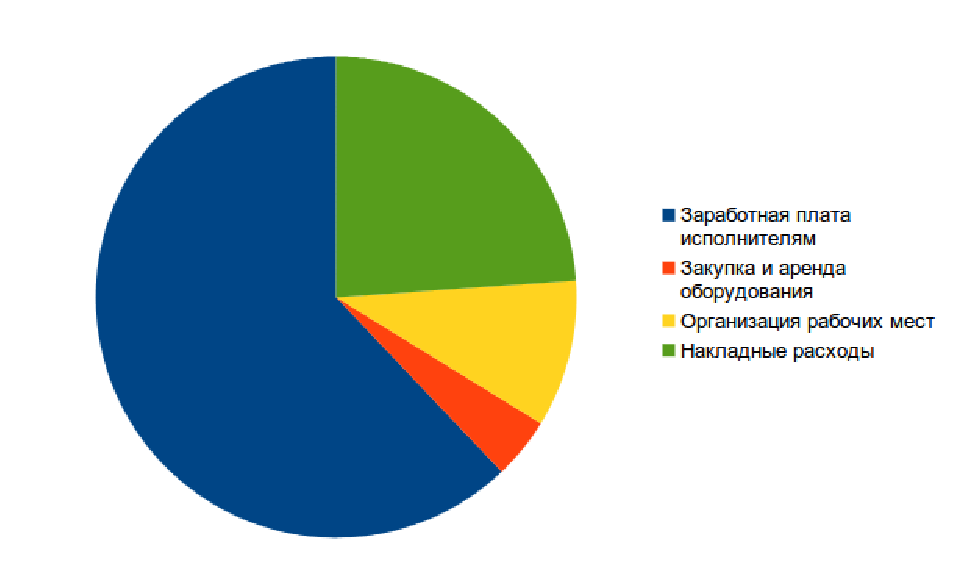
\includegraphics [scale=1] {sum_cost}
  \caption{Структура затрат проекта} 
  \label{img:sum_cost}  
\end{figure}
\FloatBarrier          % Суммарные затраты на реализацию программного проекта